\documentclass[11pt, usepdftitle=false,...]{beamer}
\usetheme{default}

\usepackage[utf8]{inputenc}
\usepackage[ngerman]{babel}
\usepackage{amsmath}
\usepackage{amsfonts}
\usepackage{amssymb}
\usepackage{graphicx}
\usepackage{pgf} 
\usepackage{caption}
\hypersetup{pdftitle=Abschlusspräsentation}
\usepackage{subcaption}
\captionsetup{compatibility=false}
\setbeamertemplate{caption}[numbered]

\author{Denis Gensh, Marcel Herm, David Krah,\\
	Eduard Kukuy, Daniel Milbaier, Richard Rudolph}
\title{
	\textbf{Abschlusspräsentation}
}
\subtitle{Workflow System für eine virtuelle Forschungsumgebung für
	Geodaten
	\vspace{-0.7cm}
	}
\logo{\pgfputat{\pgfxy(-1.7,8.0)}{\pgfbox[center,base]{
\includegraphics[scale=0.125]{images/logo.png}}}}
\institute{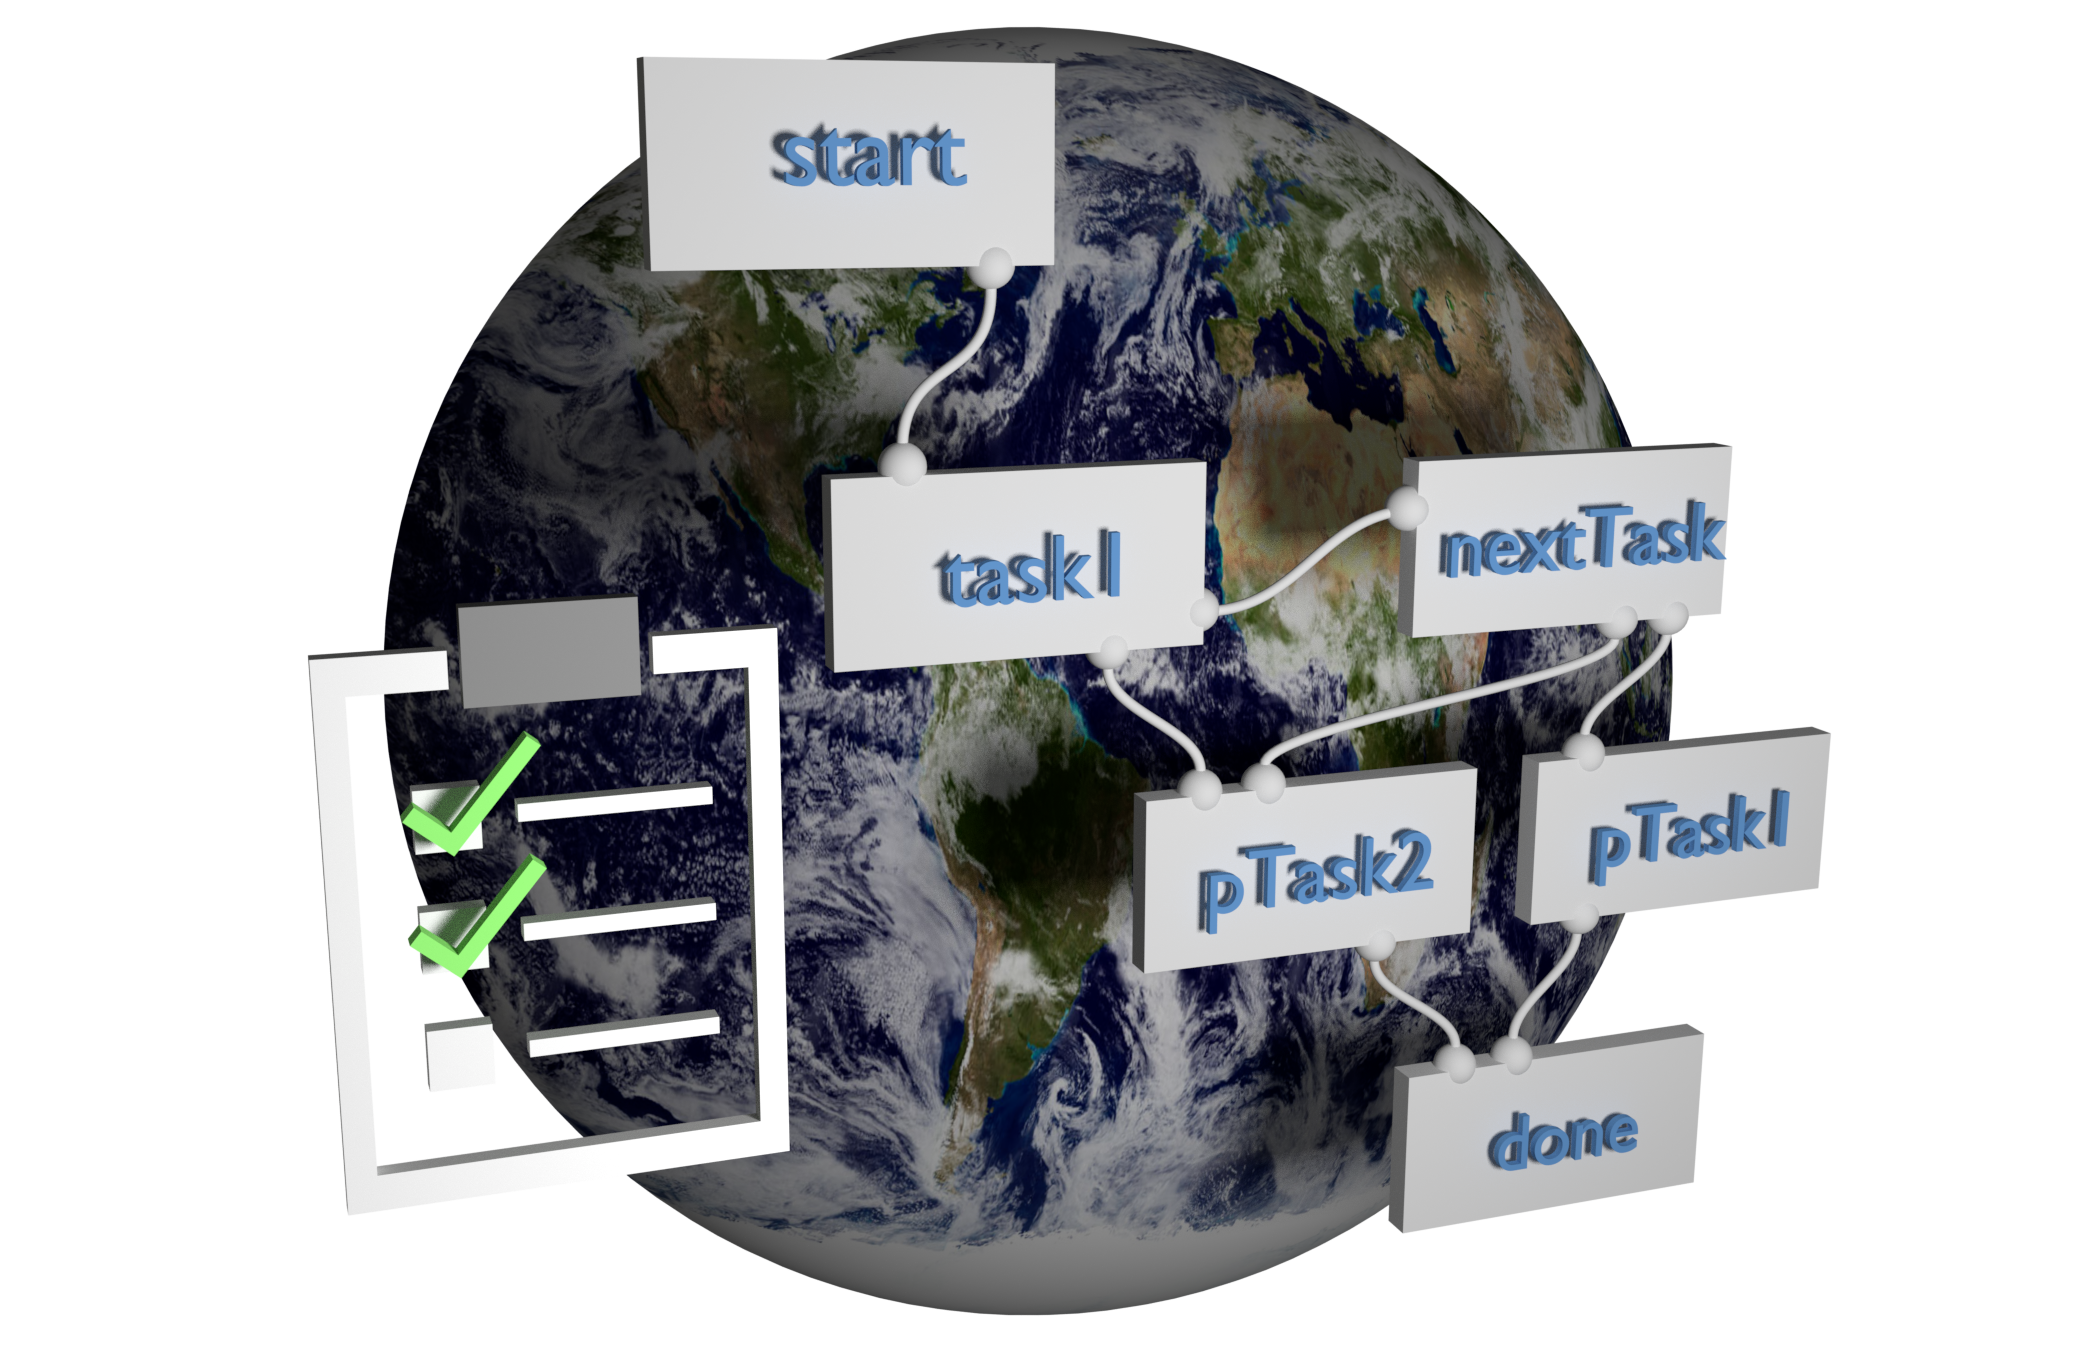
\includegraphics[height=3.5cm]{images/workflow2-tp3.png}}
\date{19. März 2018}
\subject{x}
%\setbeamercovered{transparent}
%\setbeamertemplate{navigation symbols}{}
\addtobeamertemplate{navigation symbols}{}{%
	\usebeamerfont{footline}%
	\usebeamercolor[fg]{footline}%
	\hspace{1em}%
	\insertframenumber/\inserttotalframenumber
}

\makeatletter
\setbeamertemplate{frametitle}{
	\ifbeamercolorempty[bg]{frametitle}{}{\nointerlineskip}%
	\@tempdima=\textwidth%
	\advance\@tempdima by\beamer@leftmargin%
	\advance\@tempdima by\beamer@rightmargin%
%	\hspace*{0} %%%%%%%%%%%%% For example insert shift to right
	\begin{beamercolorbox}[sep=0.5cm,left,wd=\the\@tempdima]{frametitle}
		\usebeamerfont{frametitle}%
		\vbox{}\vskip-1ex%
		\if@tempswa\else\csname beamer@ftecenter\endcsname\fi%
		\strut\insertframetitle\strut\par%
		{%
			\ifx\insertframesubtitle\@empty%
			\else%
			{\usebeamerfont{framesubtitle}\usebeamercolor[fg]{framesubtitle}\insertframesubtitle\strut\par}%
			\fi
		}%
		\vskip-3ex%
		\if@tempswa\else\vskip-.3cm\fi% set inside beamercolorbox... evil here...
	\end{beamercolorbox}%
}
\makeatother

\begin{document}
	{
		% no page #, no logo on title page
		\setbeamertemplate{footline}{}
		\setbeamertemplate{logo}{}
		\setbeamertemplate{navigation symbols}{}
		\begin{frame}
			\titlepage
		\end{frame}
	}
	
	%\maketitle
	
	
	\begin{frame}
		\frametitle{Inhaltsverzeichnis}
		\tableofcontents
	\end{frame}
	
	
	\section{Unsere Erfahrung zu PSE}
	\frame{\sectionpage}
	
	\begin{frame}{Was wir gelernt haben}
	    \begin{itemize}
	        \item Neue Programmiersprachen
	        \item Große neue Projekte durchziehen
	        \item Zusammenarbeit im Team
	    \end{itemize}
	    
	\end{frame}
	
	\begin{frame}{Feedback zum Wasserfallmodell\\ mit Rückkopplung}
	    \begin{itemize}
	        \item Gut als erstes großes Projekt
	        \item Jedoch agile Anpassungen notwendig
	    \end{itemize}
	\end{frame}
	
	
	
	\section{Live-Demo}
	\frame{\sectionpage}
	
	
	\section{Verwendete Tools}
	\frame{\sectionpage}
	
	\begin{frame}{Gitstats}
	    \begin{itemize}
	        \item 20708 Zeilen Code
	        \item 403 Commits
	    \end{itemize}
	\end{frame}
	
	\begin{frame}{Gitstats}
	    \begin{figure}[ht] 
					\centering
					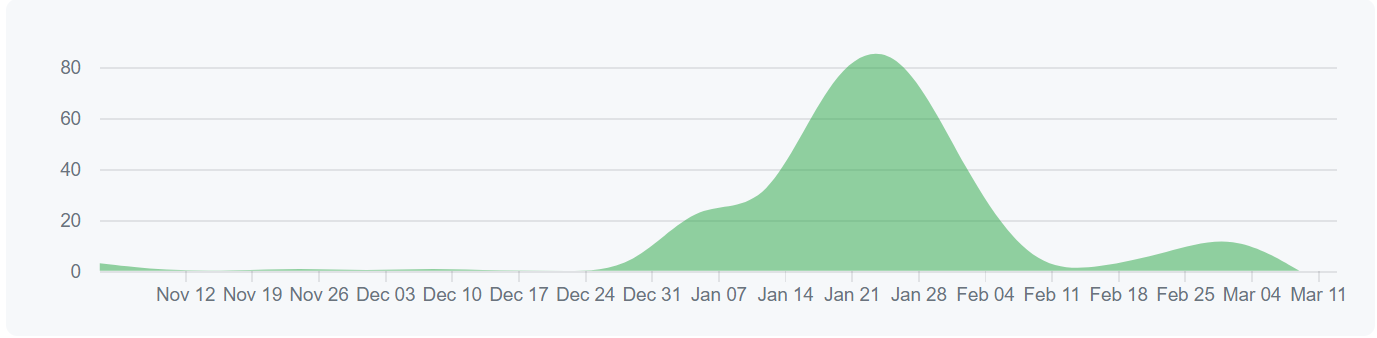
\includegraphics[width=11cm]{images/PSE_Commits.PNG}
					\label{Commits}
				\end{figure}
	\end{frame}
	
	\begin{frame}{Gitstats}
	    \begin{figure}[ht] 
					\centering
					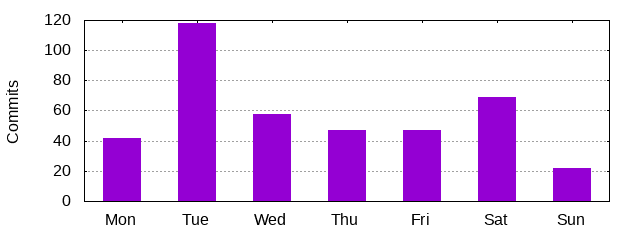
\includegraphics[width=11cm]{images/day_of_week.png}
					\label{Commits}
				\end{figure}
	\end{frame}
	
	\begin{frame}{Gitstats}
	    \begin{figure}[ht] 
					\centering
					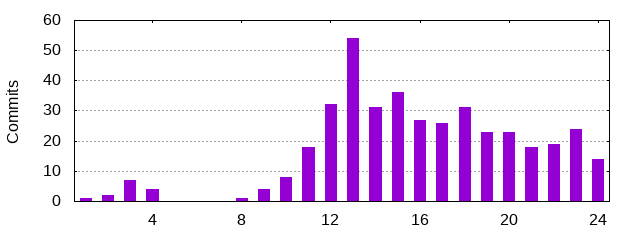
\includegraphics[width=11cm]{images/hour_of_day.png}
					\label{Commits}
				\end{figure}
	\end{frame}
	
	
	
	\begin{frame}{IDE}
	    \begin{itemize}
	        \item PyCharm
	        \item WebStorm
	        \item VSCode
	        \item Eclipse
	    \end{itemize}
	\end{frame}
	
	\begin{frame}{Dokumentation}
	    \begin{itemize}
	        \item ShareLaTeX
	        \item samepage.io
	        \item Epydoc
	        \item JSDoc
	    \end{itemize}
	\end{frame}
	    
	
	\begin{frame}
		\frametitle{}
		\centering
		\Huge Fragen?
	\end{frame}
	
\end{document}